\section{Control}

El control de robots industriales es un proceso complejo que involucra múltiples etapas para garantizar que el movimiento del robot siga de manera precisa una trayectoria deseada. En la Figura~\ref{fig:diagrama-de-robot-industrial}, se presenta un diagrama de bloques que describe este proceso, el cual puede dividirse en varias secciones fundamentales.

\textbf{Definición de valores del efector final por el usuario.} El proceso inicia cuando el usuario define los valores deseados para el efector final del robot, es decir, la parte del robot que interactúa con el entorno (por ejemplo, una pinza o una herramienta). Estos valores pueden incluir la posición, velocidad, aceleración y la trayectoria general que debe seguir el efector. Esta etapa representa las condiciones o metas que el usuario desea que el robot cumpla durante su operación.

\textbf{Planificación de trayectorias.} Una vez establecidos los valores deseados por el usuario, el sistema realiza una planificación de trayectorias. Esta etapa tiene como objetivo generar una trayectoria que sea físicamente viable, considerando las limitaciones cinemáticas y dinámicas del robot. La trayectoria no solo debe cumplir con los puntos finales deseados, sino también con parámetros como continuidad, suavidad y restricciones de velocidad y aceleración.

\textbf{Valores del efector final.} Posteriormente, se obtienen los valores específicos que describen la trayectoria del efector final. Estos incluyen no solo la posición y velocidad, sino también parámetros de orden superior como la aceleración, el \textit{jerk} (derivada de la aceleración) y el \textit{snap} (derivada del jerk), los cuales son fundamentales para evitar movimientos bruscos que puedan comprometer la estabilidad o la precisión del robot.

\textbf{Cinemática inversa.} La cinemática inversa es un proceso esencial que convierte los valores del espacio cartesiano (del efector final) a valores articulares del robot. Es decir, traduce las posiciones y movimientos deseados del efector final en los ángulos, velocidades y aceleraciones que deben alcanzar las articulaciones del robot para lograr dicha trayectoria. Este paso es fundamental para que el robot pueda ejecutar los movimientos deseados con precisión.

\textbf{Valores articulares.} Una vez realizados los cálculos de cinemática inversa, se obtiene la trayectoria de las articulaciones del robot. Estos valores incluyen la posición articular, la velocidad y la aceleración que cada articulación debe seguir para que el efector final cumpla con la trayectoria planificada. Esta información sirve como referencia para el sistema de control.

\textbf{Sistema de control.} El controlador recibe los valores articulares deseados y los compara con los valores reales obtenidos a partir de sensores. Esta comparación genera una señal de error que es procesada para determinar la señal de control adecuada (por ejemplo, el torque o fuerza que debe aplicarse en cada articulación). El objetivo del controlador es minimizar el error y asegurar que las articulaciones del robot sigan fielmente la trayectoria deseada. En muchos casos, se utilizan controladores en lazo cerrado que actualizan continuamente la señal de control en función del comportamiento real del robot.

\textbf{Dinámica del robot.} El comportamiento físico del robot está determinado por su dinámica, que incluye aspectos como la masa, la inercia, la fricción y otras fuerzas externas o internas. En el diagrama se representa mediante un sistema dinámico no lineal. La dinámica del robot responde a las señales de control aplicadas y produce el movimiento real del sistema, que a su vez es retroalimentado al controlador para seguir ajustando el comportamiento del robot.

\textbf{Sistema de lazo cerrado.} Todo el proceso descrito opera en un esquema de control en lazo cerrado, donde la información de salida (el estado actual del robot) se retroalimenta continuamente al controlador. Esta retroalimentación permite realizar ajustes en tiempo real y mejora la precisión, robustez y estabilidad del sistema de control, especialmente ante perturbaciones externas o incertidumbres en el modelo dinámico del robot.

\begin{figure}[h]
	\centering
	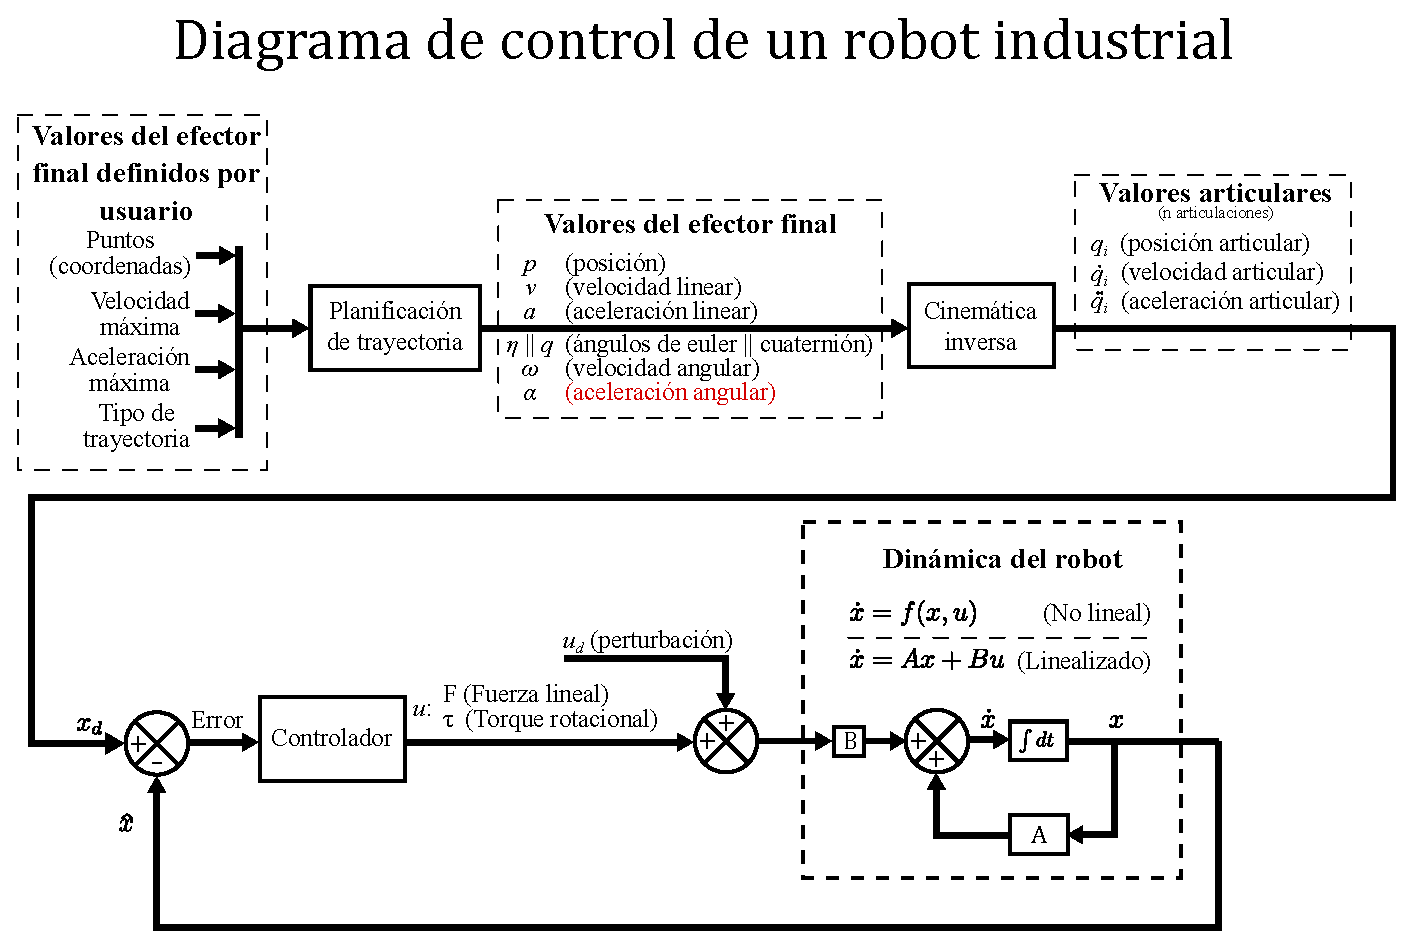
\includegraphics[width=0.55\linewidth]{img/Diagrama_robot_industrial}
	\caption{Diagrama de bloques de un robot industrial}
	\label{fig:diagrama-de-robot-industrial}
\end{figure}
